\section{Implementation Workflow}

The workflow for generating CoreDSL code from OSAL files, as depicted in Figure 4.1, involves several key stages that transform input operations into CoreDSL code suitable for integration into M2-ISA-R. The overall flow can be divided into the following steps:

\begin{figure}[h]
  \centering
  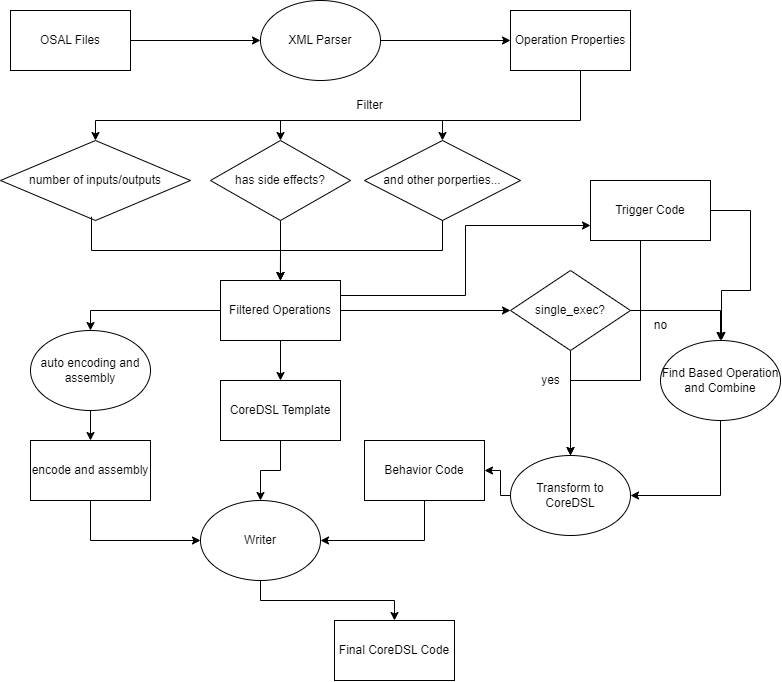
\includegraphics[width=\linewidth]{figures/flow.png}
  \caption{Implementation Flow}
\end{figure}

\section{XML Parser}

The process begins with the input OSAL (Operation Set Architecture Language) files, which contain the operation definitions. OpenASIP uses XML to define the properties and semantics of custom operations. To translate these operations into CoreDSL, we need to parse the XML representation and extract the necessary information. We developed an XML parser based on the \texttt{pandas} package in Python to read the XML files and extract the operation details.

The parser utilizes an object-oriented approach to ensure modularity and scalability. The extracted data is stored in the form of \texttt{pandas} DataFrames, which allows for efficient manipulation and filtering of the operations in the subsequent stages of processing. This structure provides flexibility for further operations, such as filtering based on input/output parameters or other properties, as required by the translation process.

\section{Operation Filtering}

The next stage involves filtering the operations based on predefined criteria. This step is crucial for identifying the operations that are suitable for further processing and transformation into CoreDSL code. The filtering process is designed to select operations that meet specific requirements, such as the number of inputs and outputs, the presence of side effects, or other characteristics that are relevant for the translation process.

\section{CoreDSL Template Generation}

The generation of the CoreDSL template involves several key steps. First, an empty CoreDSL template is created, which serves as the scaffold for defining the behavior of the custom operations. Then, the program iterates over the \textit{filtered operations} and fills in the necessary details into the template. The generation process leverages the parsed information from the XML files, including operation-specific attributes such as the number of input and output registers. The custom instructions are automatically encoded based on their properties, and the corresponding assembly code is generated.

\begin{lstlisting}[caption={CoreDSL Template},captionpos=b]
  InstructionSet OpenASIP_base extends RV32I {
    functions{
        // Inline functions for behavior
    }
    instructions {
        // Example for custom instruction
        OpenASIP_base_SHL1ADD {
            encoding: 7'b0000000 :: rs2[4:0] :: rs1[4:0] :: 3'b000 :: rd[4:0] :: 7'b0001011;
            assembly: "{name(rd)}, {name(rs1)}, {name(rs2)}";
            behavior: {
                // Behavior code will be generated here
            }
        }
        // Additional instructions will be iteratively generated
    }
  }
\end{lstlisting}

\subsection{Inline Function}

The inline functions required for custom operations are defined as part of the \textit{trigger codes} within the OpenASIP framework. Although OpenASIP provides the trigger code definition, it does not include the actual implementation of these inline functions. Fortunately, these functions are relatively simple to implement and are inserted at the beginning of the CoreDSL file. This ensures that all behavior code for custom instructions can utilize these functions during execution.

\subsection{Auto Encoding and Assembly}

The encoding process for custom instructions is handled automatically by the program. As the filtered operations are processed sequentially, each instruction is assigned an encoding that follows the RISC-V extension format. For example, instructions with two input registers (\texttt{rs1} and \texttt{rs2}) and one output register (\texttt{rd}) will be encoded in a standard 32-bit RISC-V format.

For assembly code generation, the program analyzes the XML-defined instruction attributes, such as the number of source and destination registers. Based on these attributes, it generates the corresponding assembly format string, ensuring that the generated assembly matches the intended behavior of each instruction. The following example shows how the registers are referenced in the assembly code:

\begin{lstlisting}
  assembly: "{name(rd)}, {name(rs1)}, {name(rs2)}";
\end{lstlisting}

This ensures that all operations are properly defined within the CoreDSL framework, both at the encoding level and in terms of their assembly representation.

\section{Behavior Code Generation}

The generation of behavior code for custom operations is a crucial step in translating operation semantics into executable instructions within the CoreDSL framework. This process primarily revolves around interpreting the trigger semantics provided for each operation and converting them into behavior code that can be executed by the target architecture.

\subsection{Handling \texttt{single\_execute} Operations}

Operations classified as \texttt{single\_execute} are those that involve zero or exactly one \texttt{EXEC\_OPERATION}. These operations are simpler to handle, as their semantics are either minimal or require only a single execution step. The process of generating behavior code for \texttt{single\_execute} operations is as follows:

\begin{enumerate}
    \item \textbf{Search for Trigger Code}: The program first attempts to locate the corresponding trigger code from the parsed operation semantics. This code typically contains the behavior definition for the operation.

    \item \textbf{Fallback for Missing Trigger Code}: If the trigger code is not found, the program uses a fallback approach. In this case, the tool looks for a base operation (i.e., a related or parent operation) that shares similar functionality. If a base operation is identified, its behavior code is transformed and reused. If no such base operation is available, a warning is issued, and the behavior code is generated as a placeholder or default behavior, depending on the requirements of the architecture.

    \item \textbf{Example}:
    \begin{lstlisting}
        // Example of a fallback behavior code for a missing trigger
        X[rd % RFS] = X[rs1 % RFS] + X[rs2 % RFS]; // Default operation: addition
    \end{lstlisting}
\end{enumerate}

This approach ensures that even when the exact semantics are not available, the system can still produce a working instruction that adheres to general operation principles.

\subsection{Handling Different Variable Names}

In some cases, variable names in the trigger code might differ from the expected format used in the CoreDSL framework. This is a common issue, especially when operations are defined in different contexts or environments. The tool handles this issue by:

\begin{enumerate}
    \item \textbf{Pattern Matching and Variable Mapping}: The tool applies pattern matching to identify variables in the trigger code (e.g., \texttt{rs1}, \texttt{rs2}, \texttt{rd}) and maps them to the expected format used in the target architecture. This ensures consistency in variable naming across all operations.

    \item \textbf{Renaming Strategy}: If the trigger code uses custom variable names (e.g., \texttt{temp\_reg} or \texttt{intermediate\_value}), the tool automatically replaces these with the standard naming convention used in CoreDSL (such as \texttt{X[rs1]}, \texttt{X[rs2]}, \texttt{X[rd]}). This is done using regular expressions to match and substitute variable names accordingly.

    \item \textbf{Example}:
    \begin{lstlisting}
        // Before transformation: uses custom variable names
        temp_reg = X[rs1] + X[rs2];
        intermediate_value = temp_reg * 2;

        // After transformation: standard variable names
        X[rd % RFS] = X[rs1 % RFS] + X[rs2 % RFS];
        X[rd % RFS] = X[rd % RFS] * 2;
    \end{lstlisting}
\end{enumerate}

This automatic renaming ensures that all behavior code conforms to the same format, regardless of the original trigger code's naming conventions.

\subsection{Handling Missing or Incomplete Trigger Code}

There are cases where the provided trigger code is incomplete or missing certain details, such as variable initialization or conditional checks. To handle these situations, the tool applies several strategies:

\begin{enumerate}
    \item \textbf{Default Values for Missing Variables}: If a required variable is missing or uninitialized in the trigger code, the tool inserts default values or initialization based on the context of the operation. For instance, if a result register (\texttt{rd}) is not initialized, it may be set to a default value like zero or an identity element (e.g., 1 for multiplication).

    \item \textbf{Handling Conditional Logic}: If the trigger code includes conditional statements (e.g., \texttt{if} conditions) without complete implementation, the tool generates the necessary control flow structures. For example, if a condition involves checking the value of a register, the tool ensures that the check is properly implemented and that the code handles both the true and false branches.

    \item \textbf{Example}:
    \begin{lstlisting}
        // Incomplete conditional logic
        if (X[rs2] == 0) {
            // Missing else branch
        }

        // Completed by the tool
        if (X[rs2 % RFS] == 0) {
            X[rd % RFS] = 0;  // Handle divide by zero
        } else {
            X[rd % RFS] = X[rs1 % RFS] / X[rs2 % RFS];  // Normal division
        }
    \end{lstlisting}
\end{enumerate}

By filling in missing parts of the code, the tool ensures that the behavior of the instruction remains consistent and functional.

\subsection{Handling Other Corner Cases}

In addition to the common cases mentioned above, the tool also addresses several corner cases that may arise during behavior code generation:

\begin{enumerate}
    \item \textbf{Multiple \texttt{EXEC\_OPERATION} Cases}: If an operation involves multiple \texttt{EXEC\_OPERATION} statements, the tool concatenates the behavior of these operations, ensuring that all steps are executed in the correct order. For example, if an operation involves both a shift and an addition, the tool ensures that both operations are included in the final behavior code.

    \item \textbf{Complex Trigger Semantics}: For operations with complex trigger semantics (e.g., involving multiple registers or advanced arithmetic operations), the tool decomposes the trigger code into manageable steps and generates the corresponding behavior code. This may involve splitting a single line of code into multiple steps to ensure clarity and correctness.

    \item \textbf{Error Handling}: In situations where runtime errors are defined (e.g., division by zero), the tool ensures that appropriate error handling mechanisms are inserted into the behavior code. This includes raising errors or returning safe default values when an error condition is detected.
\end{enumerate}

\subsection{Final Behavior Code Generation}

The final behavior code is generated by combining the transformed trigger code, any required fallback operations, and additional corner case handling. This ensures that each operation is fully defined within the CoreDSL framework and can be executed correctly on the target architecture. The behavior code is then inserted into the CoreDSL template, completing the generation process.

\begin{lstlisting}
// Example of final behavior code
if (X[rs2 % RFS] == 0) {
    X[rd % RFS] = 0;  // Handle divide by zero
} else {
    X[rd % RFS] = X[rs1 % RFS] / X[rs2 % RFS];
}
X[rd % RFS] = X[rd % RFS] + 1;  // Additional operation
\end{lstlisting}

This process ensures that all custom operations are correctly implemented and optimized for their respective architectures, regardless of the complexity of the trigger semantics or the specific requirements of the operation.
